\section{Proposed Methods}


% \begin{frame}{Good-old BERT}

%   \begin{itemize}
%     \item BERT has long been used to classify texts.
%     \item Even with the challenges posed by toxic content, we wish to experiment with the classic method of using BERT with a classifier head.
%   \end{itemize}

% \end{frame}


\begin{frame}{Classification with KNNs}

  \begin{itemize}
    \item This approach maintains a vector database of toxic examples.
    \item When we get a new input, we use the vector database to extract k-nearest-neighbours toxic examples.
    \item We then use these examples for k-shot prompting.
    \item For classification, we can either use a transformer with a classifier head or an API call to an LLM (for example, GPT) to get a "yes" or "no" output.
  \end{itemize}
    
\end{frame}


\begin{frame}{Classification with KNNs}

  \begin{figure}
    \centering
    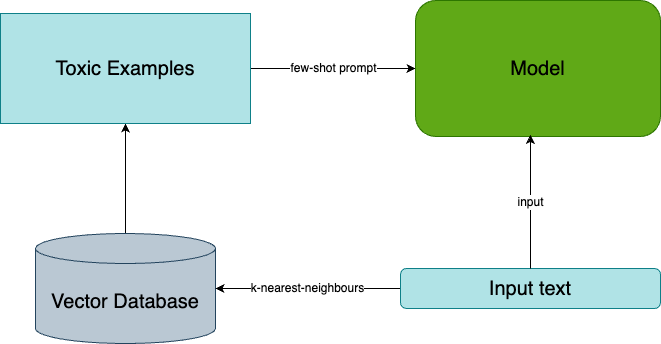
\includegraphics[width=0.8\linewidth]{images/architecture.png}
    \caption{Architecture}
  \end{figure}

\end{frame}
